% PressureResponse2q.tex

\resizebox{!}{0.3\textwidth}{
	\begin{tikzpicture}
		\only<1>{
			\node[anchor=south west,inner sep=0] (image) at (0,0)%
				{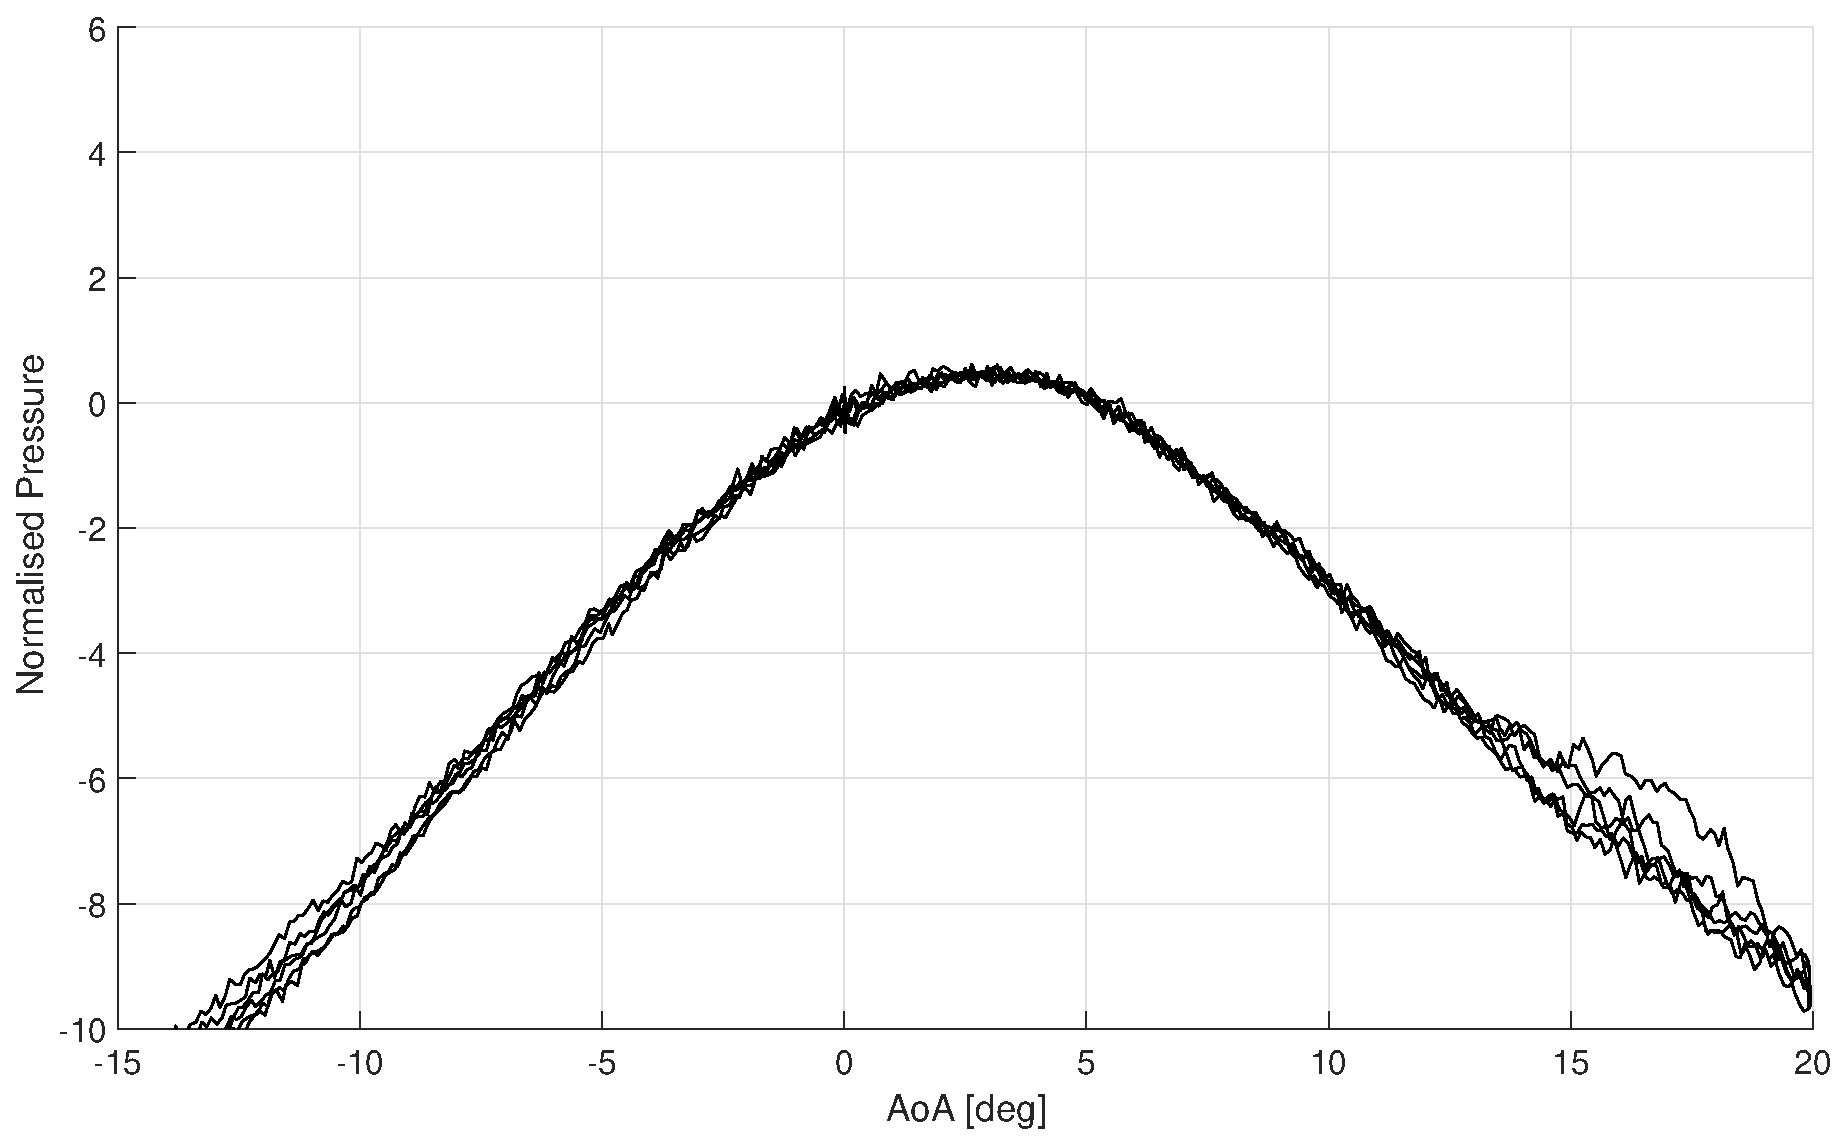
\includegraphics[width=\textwidth]{DistDataSet_P01.eps}};
		}
		\only<2>{
			\node[anchor=south west,inner sep=0] (image) at (0,0)%
				{\includegraphics[width=\textwidth]{DistDataSet_P02.eps}};
		}
		\only<3>{
			\node[anchor=south west,inner sep=0] (image) at (0,0)%
				{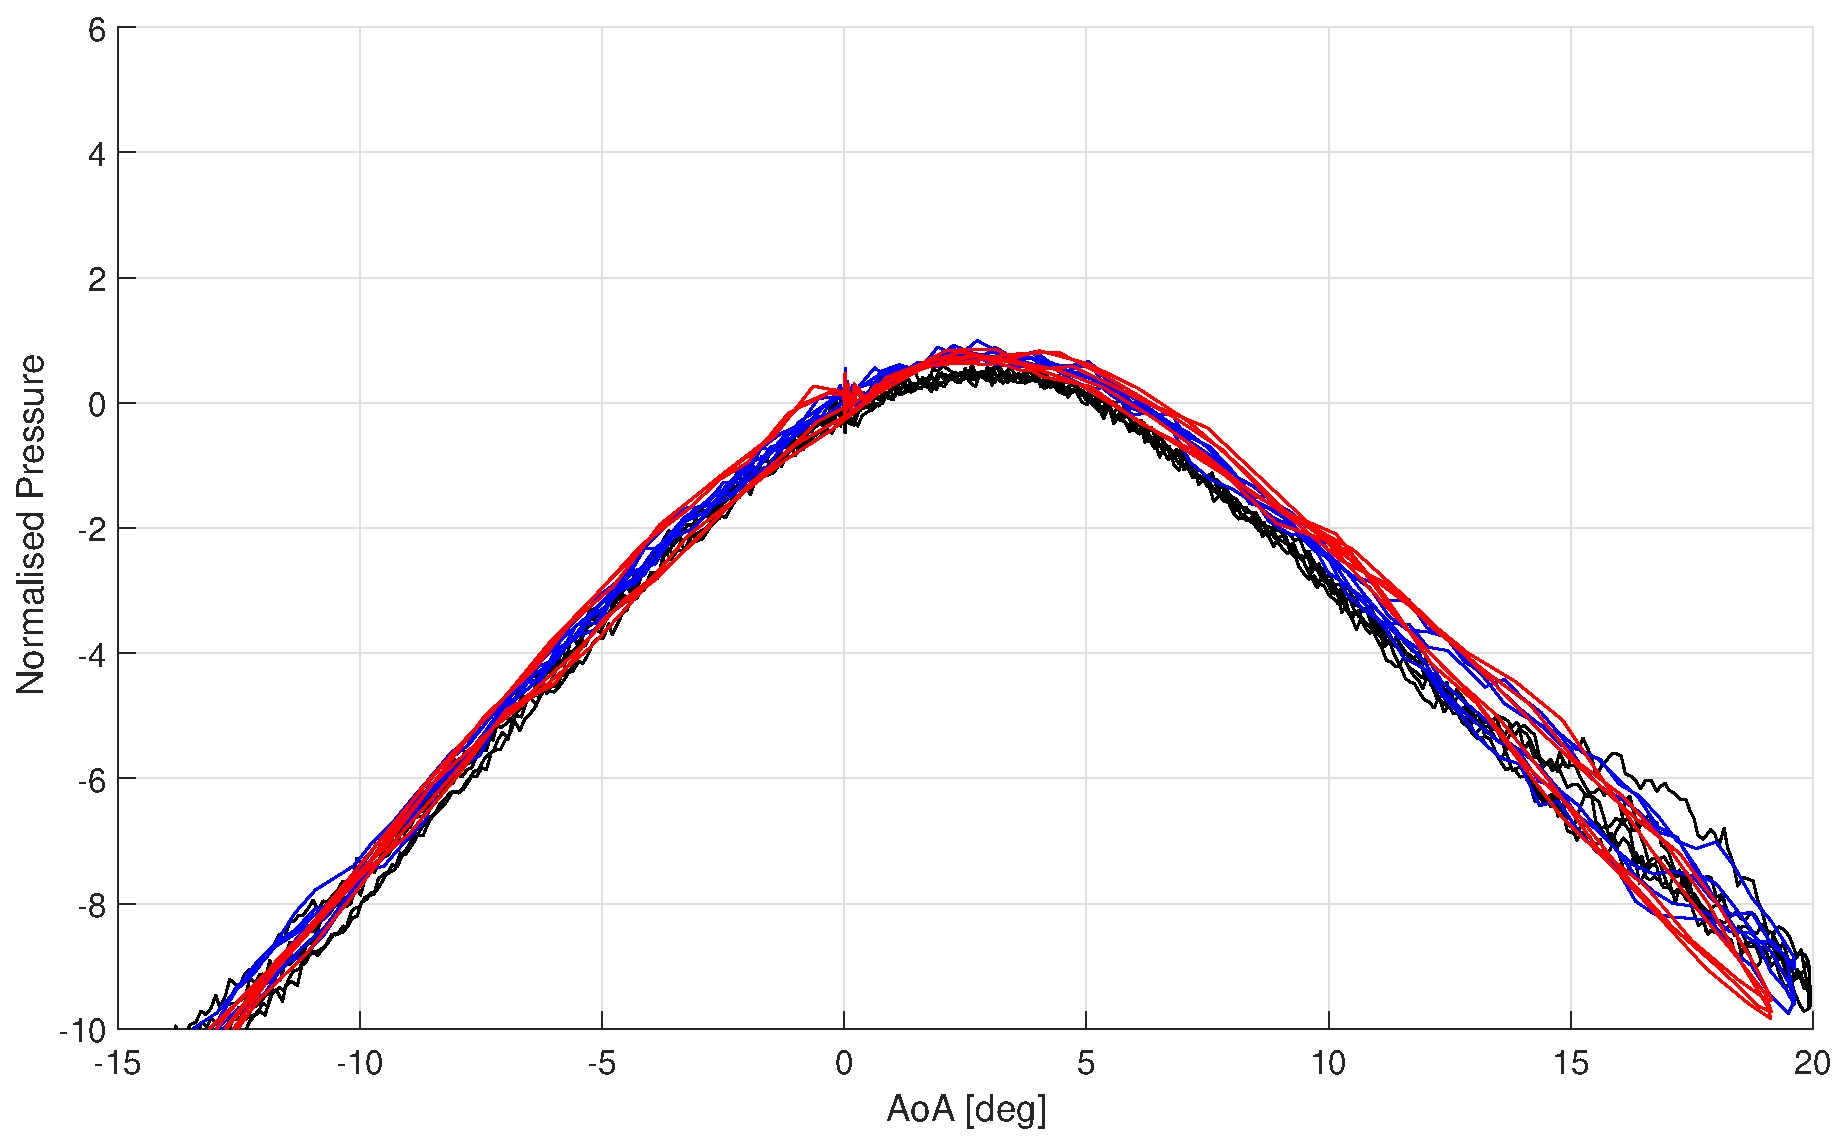
\includegraphics[width=\textwidth]{DistDataSet_P03.eps}};
		}
		\only<4>{
			\node[anchor=south west,inner sep=0] (image) at (0,0)%
				{\includegraphics[width=\textwidth]{DistDataSet_P04.eps}};
		}
		\only<5>{
			\node[anchor=south west,inner sep=0] (image) at (0,0)%
				{\includegraphics[width=\textwidth]{DistDataSet_P05.eps}};
		}
		\only<6>{
			\node[anchor=south west,inner sep=0] (image) at (0,0)%
				{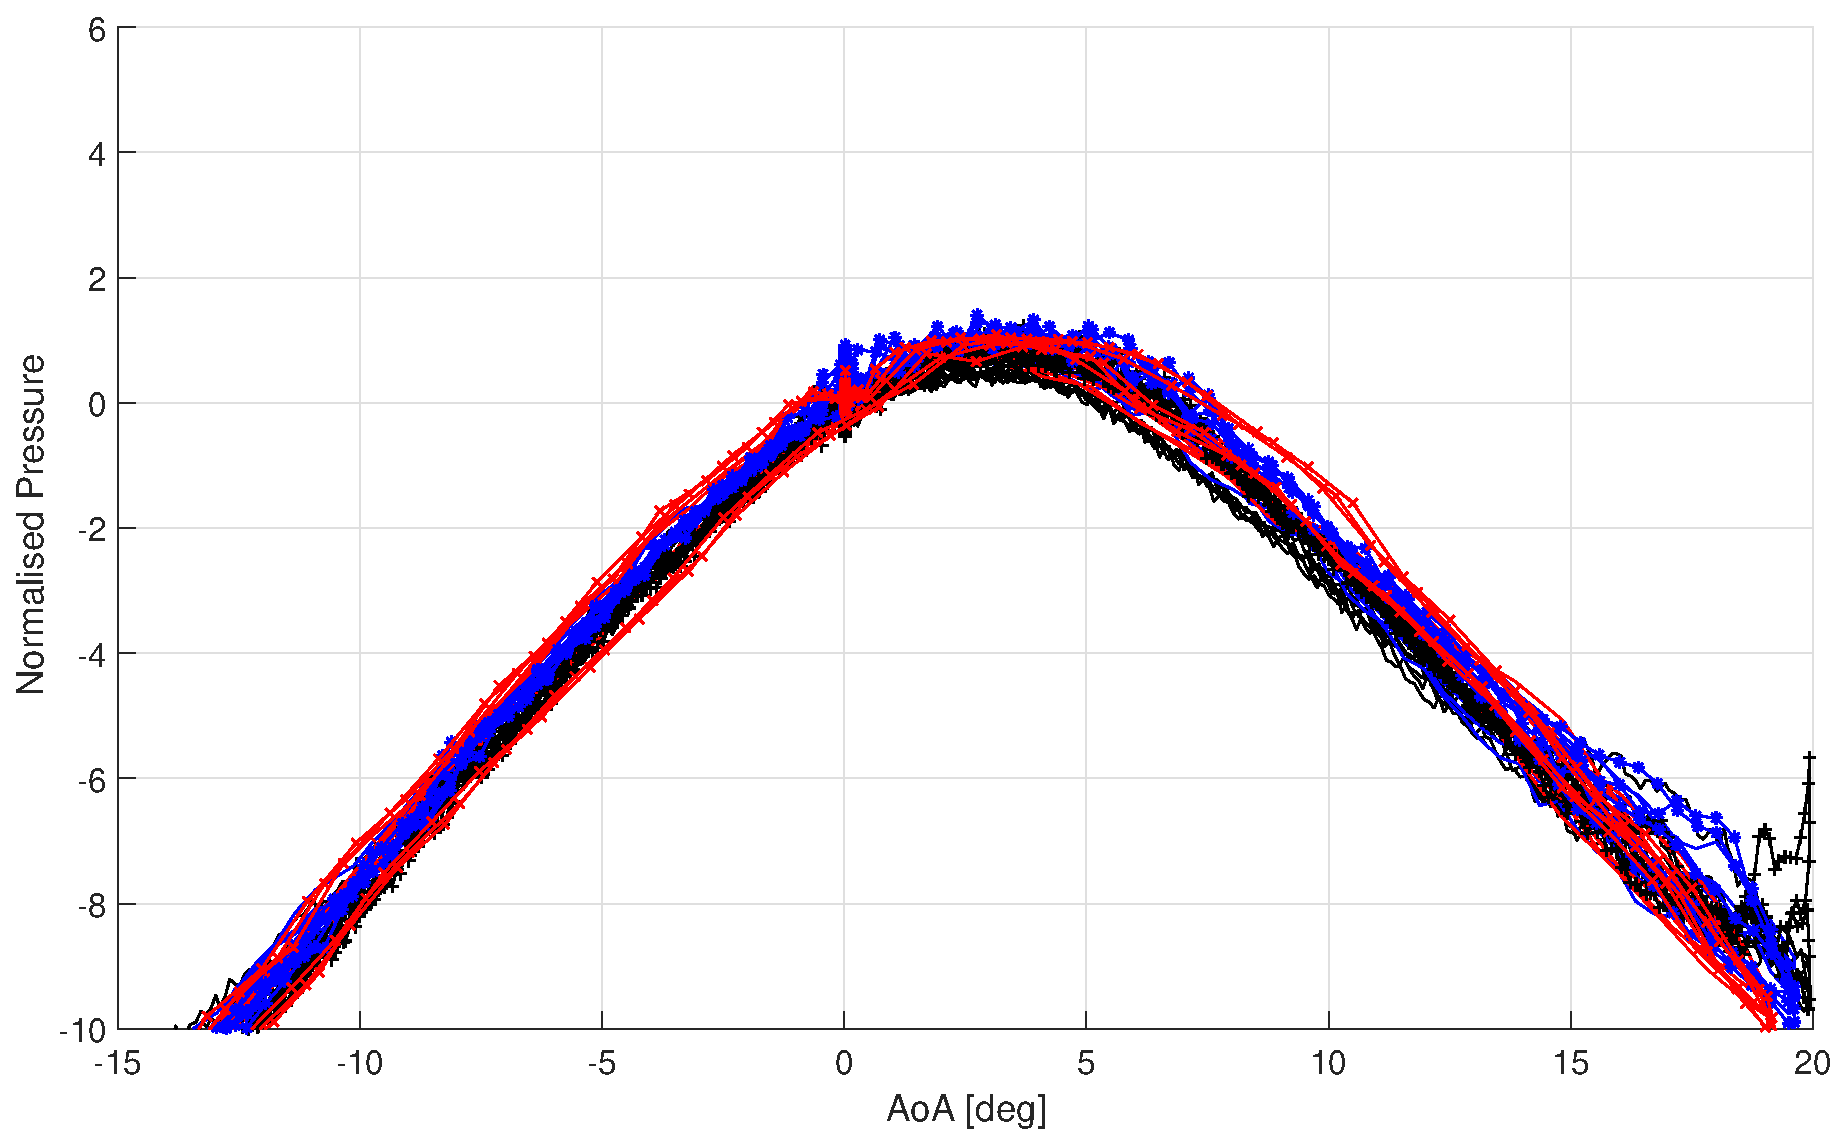
\includegraphics[width=\textwidth]{DistDataSet_P06.eps}};
		}
		% Define scope with 'image' dimensions as reference
		\begin{scope}[x={(image.south east)},y={(image.north west)}]
			%\draw[help lines,xstep=.05,ystep=.05] (0,0) grid (1,1);
			%\foreach \x in {0,1,...,9} { \node [anchor=north] at (\x/10,0) {0.\x}; }
			%\foreach \y in {0,1,...,9} { \node [anchor=east] at (0,\y/10) {0.\y}; }
			
		\end{scope}
	\end{tikzpicture}
}